\section{Modeling method application to a TLP generator}
\label{sec:tlp-modeling}

% Illustrate the method with a practical case
The methodology described previous (section \ref{sec:esd-modeling}) is applied to the \gls{tlp} bench at NXP laboratory in Toulouse.
It is a good illustration on how to use the library of models for simulating a complete system.
Also, this particular testbench is widely used in NXP for characterizing and testing products.
The model described hereafter is used for instance to validate non-linear frequency model of passive devices.

% Describe the approach
To demonstrate its accuracy, the bench model is verified with an extensive simulation versus measurement comparison flow.
First, its behavior is measured under different loads and at different charging amplitudes.
The setup is identical for each simulation and measurement and is given Fig. \ref{fig:setup-cz-tlp-model}.

\begin{figure}[!h]
  \centering
  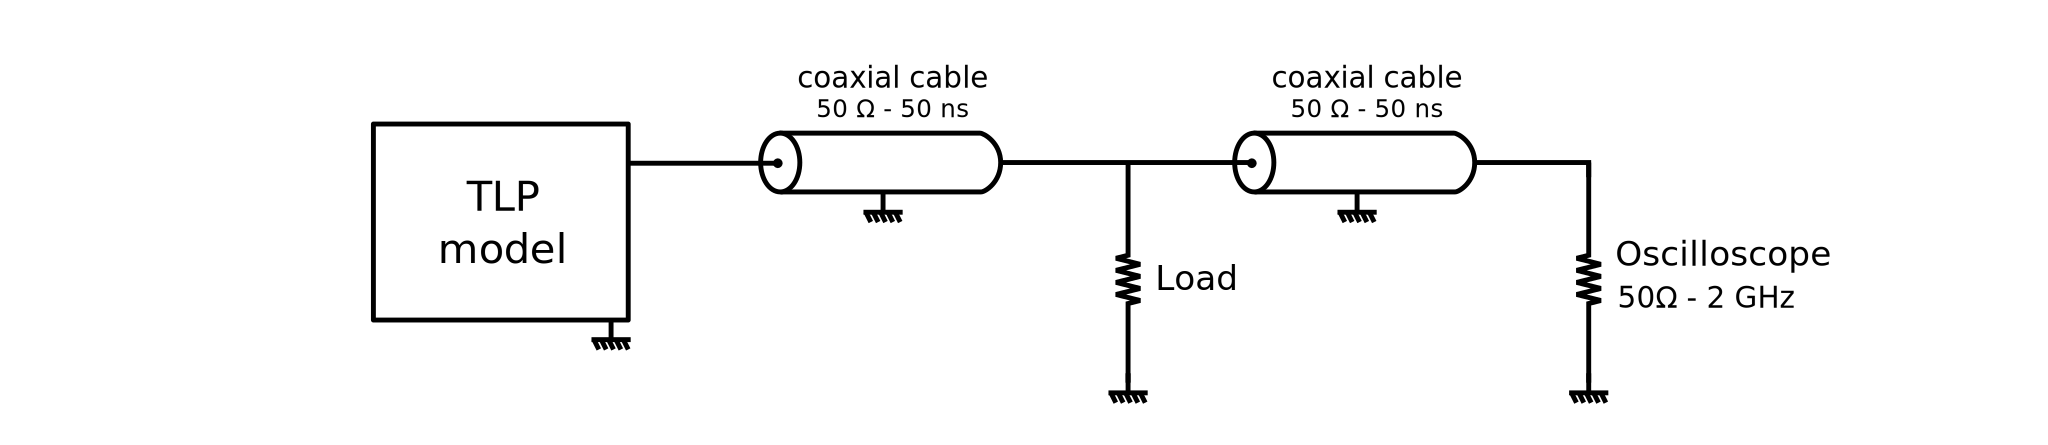
\includegraphics[width=\textwidth]{src/2/figures/tlp_characterization_setup.pdf}
  \caption{Characterization setup of the TLP}
  \label{fig:setup-cz-tlp-model}
\end{figure}

% Continue describing the approach
All the recorded time-domain waveforms serve as a reference for the modelling.
The list of test loads is constituted of resistors, capacitors and inductors of different values.
Pictures of the generator environment, its internal circuitry, and its schematic are also very valuable.
Then, a first version of the testbench model is build, taking into account elements what physically exists.
It is tested with a first \gls{spice} simulation for a resistive load and charging voltage, and waveforms are compared against measurements.
If results correlate, the validation is continued with another load or another amplitude.
If results don't correlate, the model needs corrections.
Usually, some part of the curve will match the measurement, but others won't and call for improvements.
It can be convenient to try improving a single part of the waveform at a time.
Properties of time-domain reflectometry are helpful for locating where the model needs adjustements.
Indeed, with \gls{tdr}, a portion of the curve in time corresponds to a physical location inside the system.
If the fall time of the pulse is wrong for instance, then it can mean that some device that smoothes the discharge is missing at the far end of the discharge cable.
It is also very convenient to observe pictures of the system while building the model, because some small elements might easily be missed out or forgotten from the preliminary observation, yet they might impact waveforms a lot.
If some minor sections of the curves really cannot be matched using the system schematic as reference, then parasitic devices can be added.
All of these steps should quickly converge on an accurate ESD model.

\begin{figure}[!h]
  \centering
  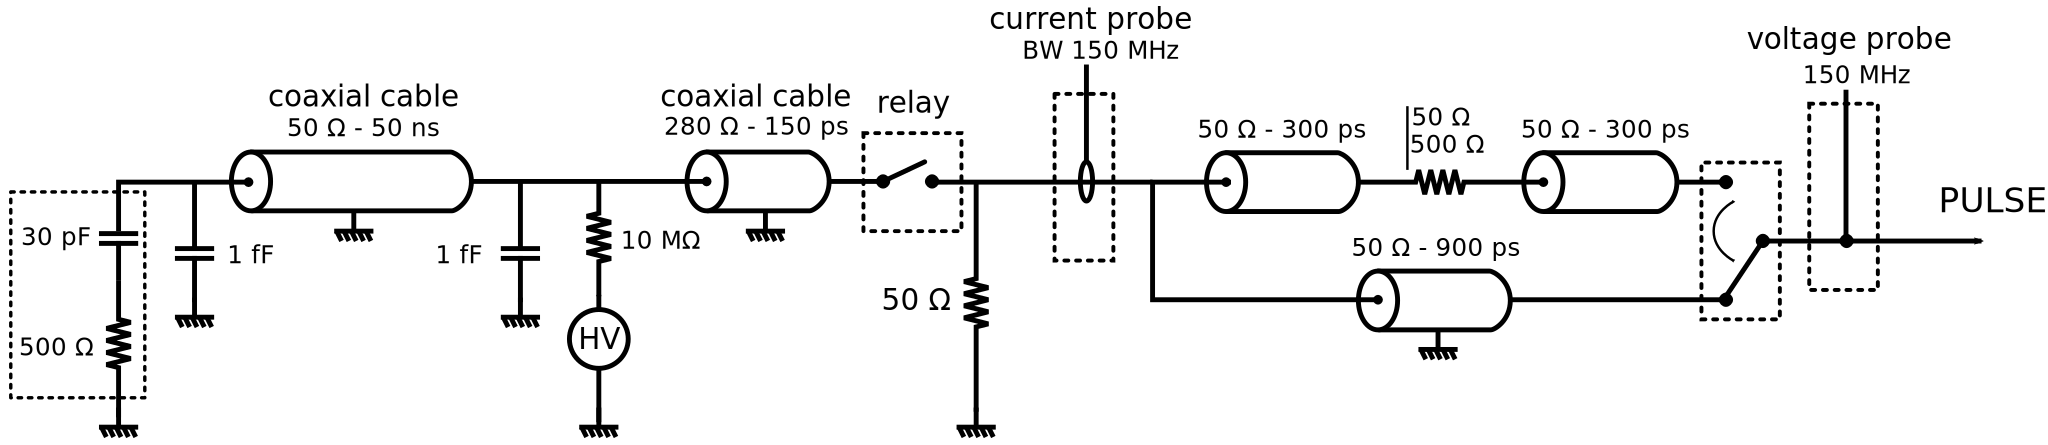
\includegraphics[width=\textwidth]{src/2/figures/complete_nxp_tlp_model.pdf}
  \caption{Complete model of NXP laboratory's TLP generator}
  \label{fig:complete-tlp-model}
\end{figure}

% Explain how the model, how it was constructed
The complete model is detailed in Fig. \ref{fig:complete-tlp-model}.
Similarly to all TLPs, the principle of operation is rather straightforward.
Initially, the relay is left open while the 50ns coaxial cable on the left is being charged by the high voltage \gls{dc} supply.
The 10 M\textOmega{} resistor ensures that the cable charges slowly to avoid oscillations, and isolates the high voltage supply from the pulse.
The two $1 fF$ capacitors placed at each end of the discharge cable help the simulator respect the initial condition for the charging voltage.
The cable is pre-charged to accelerate the simulation.
After the relay, a 50 \textOmega{} resistor can be found, intended as an attenuator.
Despite having a value of 50\textOmega{} like the coaxial cables, this resistor creates an impedance mismatch.
It is the perfect illustration of a small element that is easily missed out but impacts waveforms a lot.
A current probe is connected immediately after the attenuator, and a voltage probe is connected at the output of the generator.
Position of the probes are important as well, to reproduce the timeshift between them.
The short transmission line represented by 150 ps coaxial cables is a piece of barenaked wires.
It creates impedance mismatches because it has an estimated characteristic impedance of 280 \textOmega{}.
Finally, two discharge paths are possible inside the generator depending on the configuration of the switch on the output.
The direct path is at the bottom, where the pulse goes straight out from the generator.
The top path provides a series resistance that limits the discharge current.

% Detail a first comparison with 25 ohms
A first comparison between measurement and simulation is given in Fig. \ref{fig:comparison-tlp-load}.
With a 25\textOmega{} resistor and a charging voltage of 500V, 4.5A (I\textsubscript{TLP}) of current and 125mV (V\textsubscript{TLP}) are recorded.
The ratio of V\textsubscript{TLP}/I\textsubscript{TLP} between 40 ns to 100 ns is equal to 25\textOmega{} as expected.
Until 220 ns, both curves match closely.
After this time, some differences appear due to the bouncing back and forth of the pulse inside the system, and the accumulation of model errors.
However, most ESD investigations focus on the main part of the discharge under 120 ns.

\begin{figure}[!h]
  \centering
  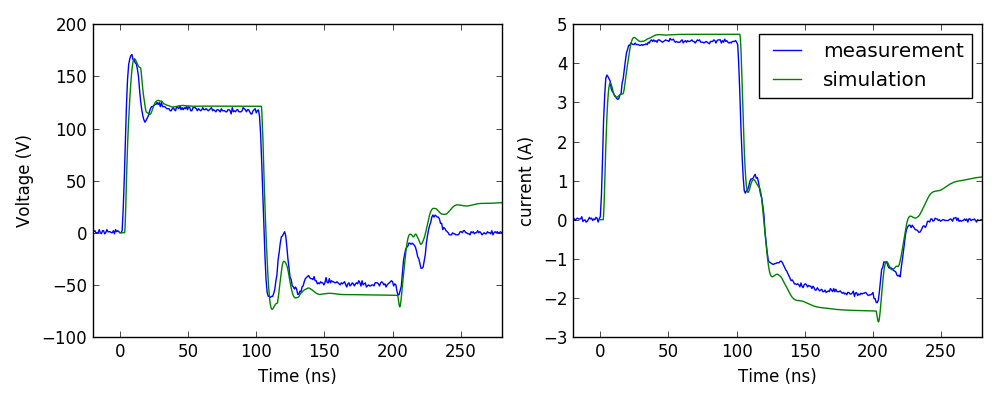
\includegraphics[width=\textwidth]{src/2/figures/tlp_comparison_R25_500V.png}
  \caption{Voltage and current waveforms comparison - 500 V charging voltage on 25\textOmega{}}
  \label{fig:comparison-tlp-load}
\end{figure}

% Second comparison with a short circuit
Same comparison is performed on a short circuit in Fig. \ref{fig:comparison-tlp-short}.
The goal is to test the extreme conditions where the model is going to be used.
As expected the voltage is null and the current is close to the maximum 10A supplied by the TLP (500 V through 50\textOmega{}).
At 120 ns, a large difference is observed between the two curves.
It is actually a measurement issue due to the oscilloscope clamping amplitude outside the observation window.
Because this is a limitation of the equipment, it is not modelled inside the simulation.

\begin{figure}[!h]
  \centering
  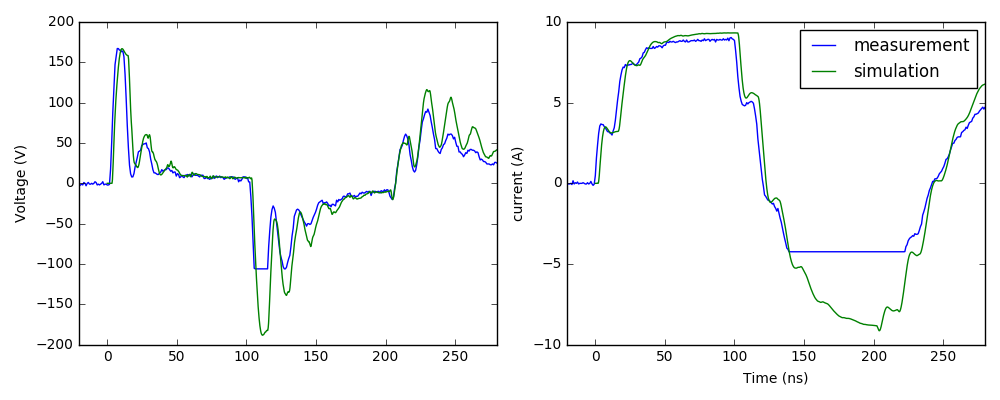
\includegraphics[width=\textwidth]{src/2/figures/tlp_comparison_short_500V.png}
  \caption{Voltage and current waveforms comparison - 500 V charging voltage on a short circuit}
  \label{fig:comparison-tlp-short}
\end{figure}

% Third comparison on an open circuit
Finally, the process is repeated on an open circuit in Fig. \ref{fig:comparison-tlp-open}.
Observations are similar to the previous figures.
The voltage is recorded at 220V, corresponding to a bit less than half the TLP charging voltage.
For an ideal TLP, the value would be exactly 250V.
Due to the 50\textOmega{} resistor between signal and ground inside this TLP, the voltage is slightly lower.
The current is close to 0A because the load is an open circuit and does absorb current.
Between 100ns and 120ns, the same clamped measurement issue than previously is observed on the current waveform.

\begin{figure}[!h]
  \centering
  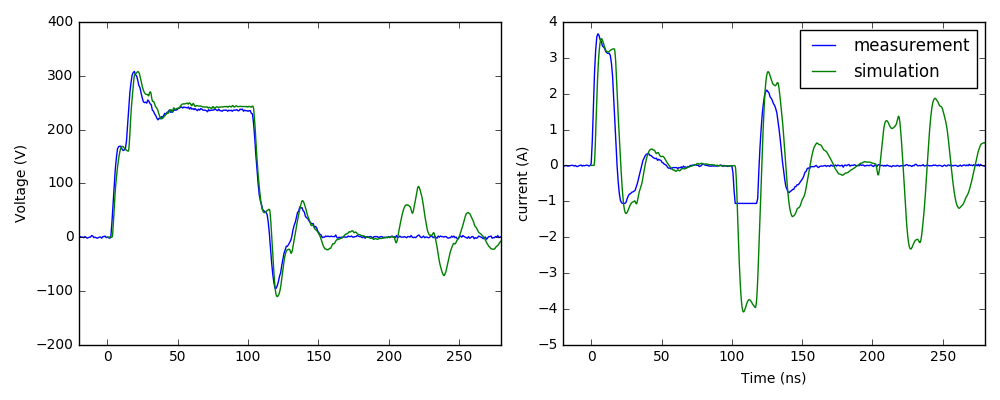
\includegraphics[width=\textwidth]{src/2/figures/tlp_comparison_open_500V.png}
  \caption{Voltage and current waveforms comparison - 500 V charging voltage on open circuit}
  \label{fig:comparison-tlp-open}
\end{figure}

% Fourth load is capacitive
So far, only resistive loads were tested.
Capacitors are interesting to validate models with non real impedance.
The response of the generator on a 1nF capacitor is given in Fig. \ref{fig:comparison-tlp-capa}.
Between 40 ns and 100 ns, voltage and current are not stable, however measurement and simulation correlate well.
This is very interesting because it validates the behavior of the generator in dynamic regime, with large varying signals.
The near-linear voltage curve is due to the capacitor being charged at nearly constant current by the TLP.
The slope of this linear curve is directly related to the capacitor value.

\begin{figure}[!h]
  \centering
  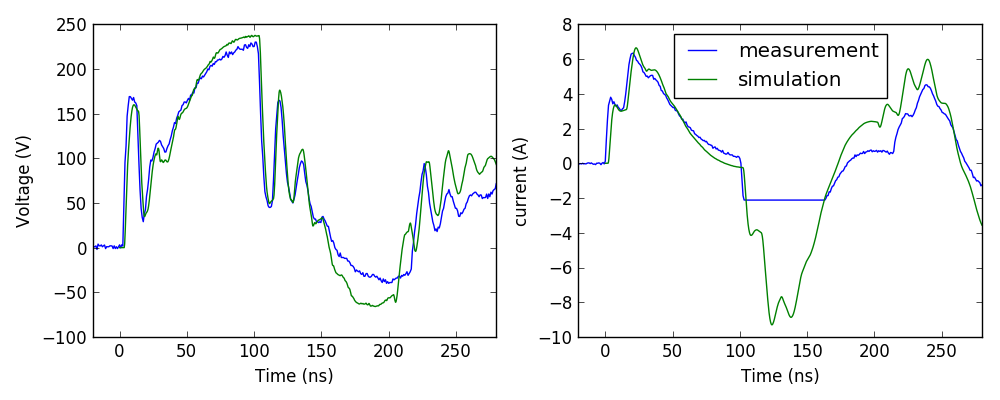
\includegraphics[width=\textwidth]{src/2/figures/tlp_comparison_1nF_500V.png}
  \caption{Voltage and current waveforms comparison - 500 V charging voltage on a 1nF capacitor}
  \label{fig:comparison-tlp-capa}
\end{figure}

% More validations in Annex
More simulation and validation curves are provided in Annex \ref{apx:tlp-validation-curves}, for different loads and amplitudes.
The goal of all those validation is to verify the model at both nominal and boundary conditions.
Overall, the model is good and fits very well the measurements, demonstrating the validity of the modelling method.
